\documentclass[12pt]{article}
\usepackage[margin=1in]{geometry}
\usepackage{amsmath}
\usepackage{xcolor}
\usepackage{tikz}
\usepackage{menukeys}
\parindent=0pt
\begin{document}

\section*{Introduction}

Commands are entered in the following field.

\begin{center}
\begin{tikzpicture}
\node at (0,0) {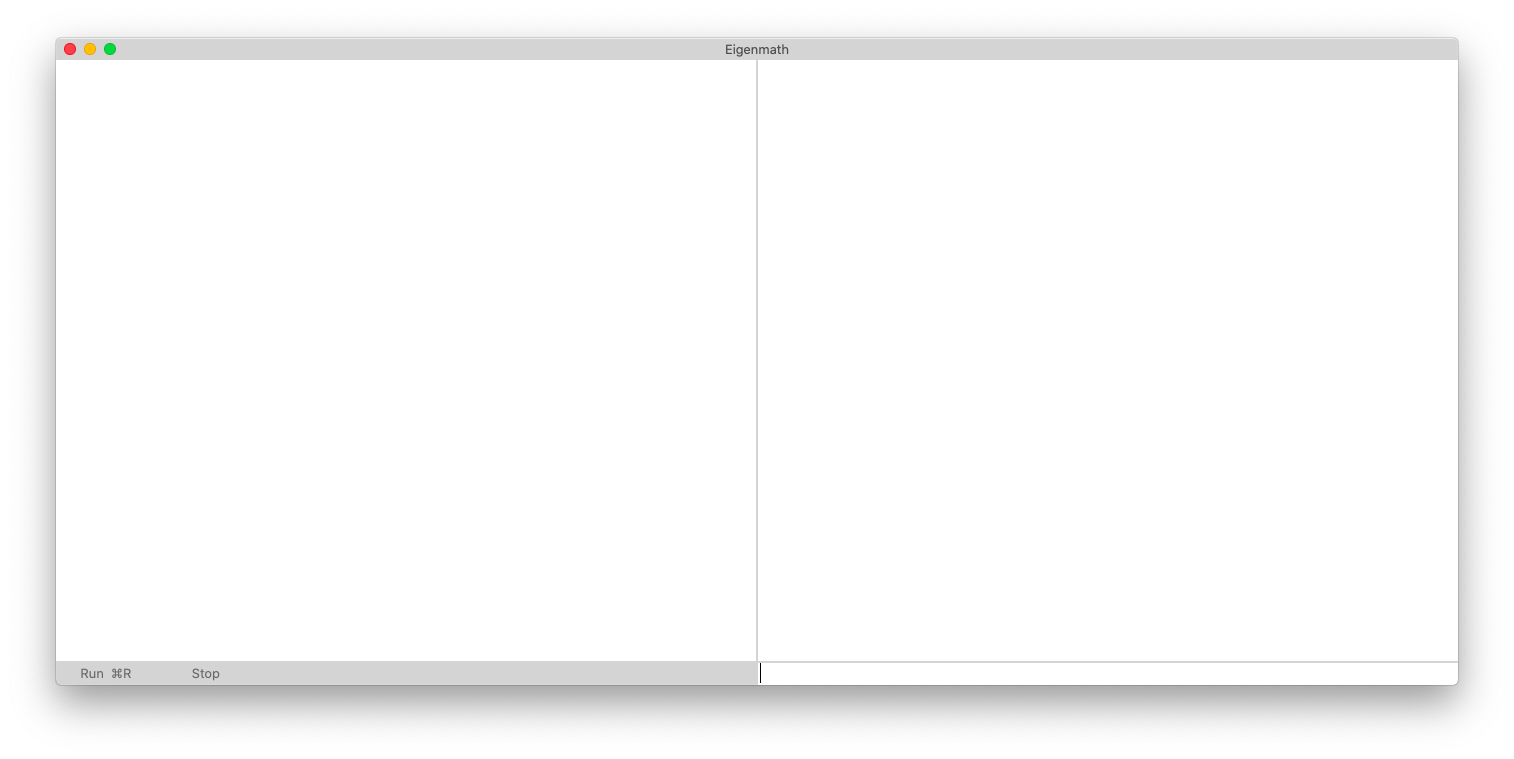
\includegraphics[scale=0.18]{screenshot.png}};
\draw[red,thick] (2.2,-1.9) ellipse (2.5cm and 0.4cm);
\end{tikzpicture}
\end{center}

Multiple commands can be put together in a script.
Scripts are run by clicking the Run button.

\begin{center}
\begin{tikzpicture}
\node at (0,0) {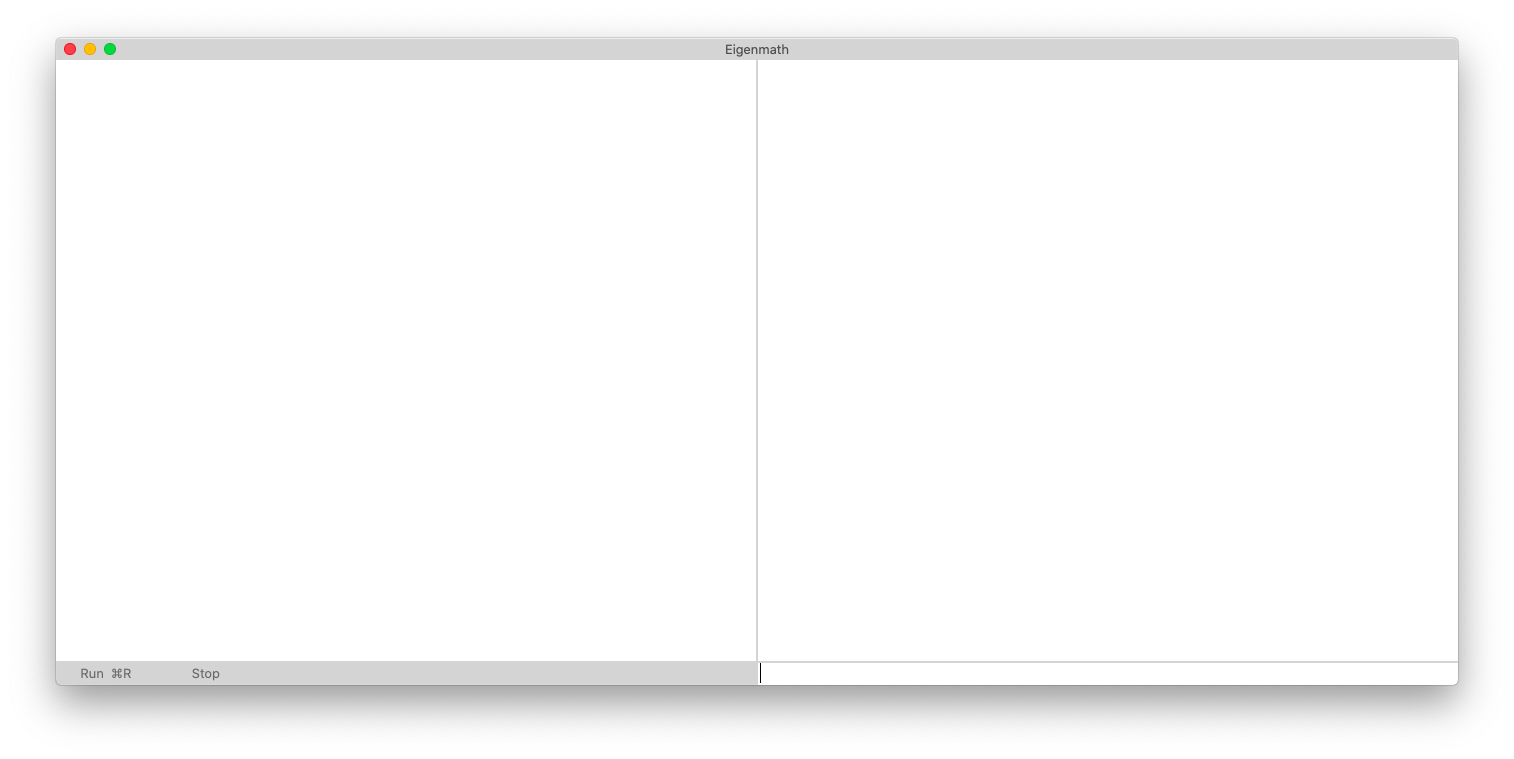
\includegraphics[scale=0.18]{screenshot.png}};
\draw (-2.2,0.1) node {Scripts go here};
\end{tikzpicture}
\end{center}

After a script runs, all of the results are available in command mode.

\bigskip
To print or copy results, click in the result field.
Then press \cmd$\,$P to print, \cmd$\,$C to copy to the clipboard.

\bigskip
Note: Eigenmath expects Times New Roman and Times New Roman Italic fonts
to be the standard macOS fonts that include special symbols and Greek letters.
See the following link for correcting font problems.

\bigskip
{\scriptsize
https://support.apple.com/guide/font-book/restore-fonts-that-came-with-your-mac-fb34862/mac
}

\newpage

In the following examples, user input is shown in blue.
The result is shown in black.

\bigskip
Example 1. Compute $212^{17}$.

{\color{blue}
\begin{verbatim}
212^17
\end{verbatim}}

$3529471145760275132301897342055866171392$

\bigskip
Example 2. Compute $212^{17}$ and save as $N$.
Then display the value of $N$.

{\color{blue}
\begin{verbatim}
N = 212^17
N
\end{verbatim}}

$N=3529471145760275132301897342055866171392$

\bigskip
Example 3. Compute the 17th root of $N$.

{\color{blue}
\begin{verbatim}
N^(1/17)
\end{verbatim}}

$212$

\end{document}
